\section{Related Work}\label{sec:Background}

\begin{figure}[t]
\centerline{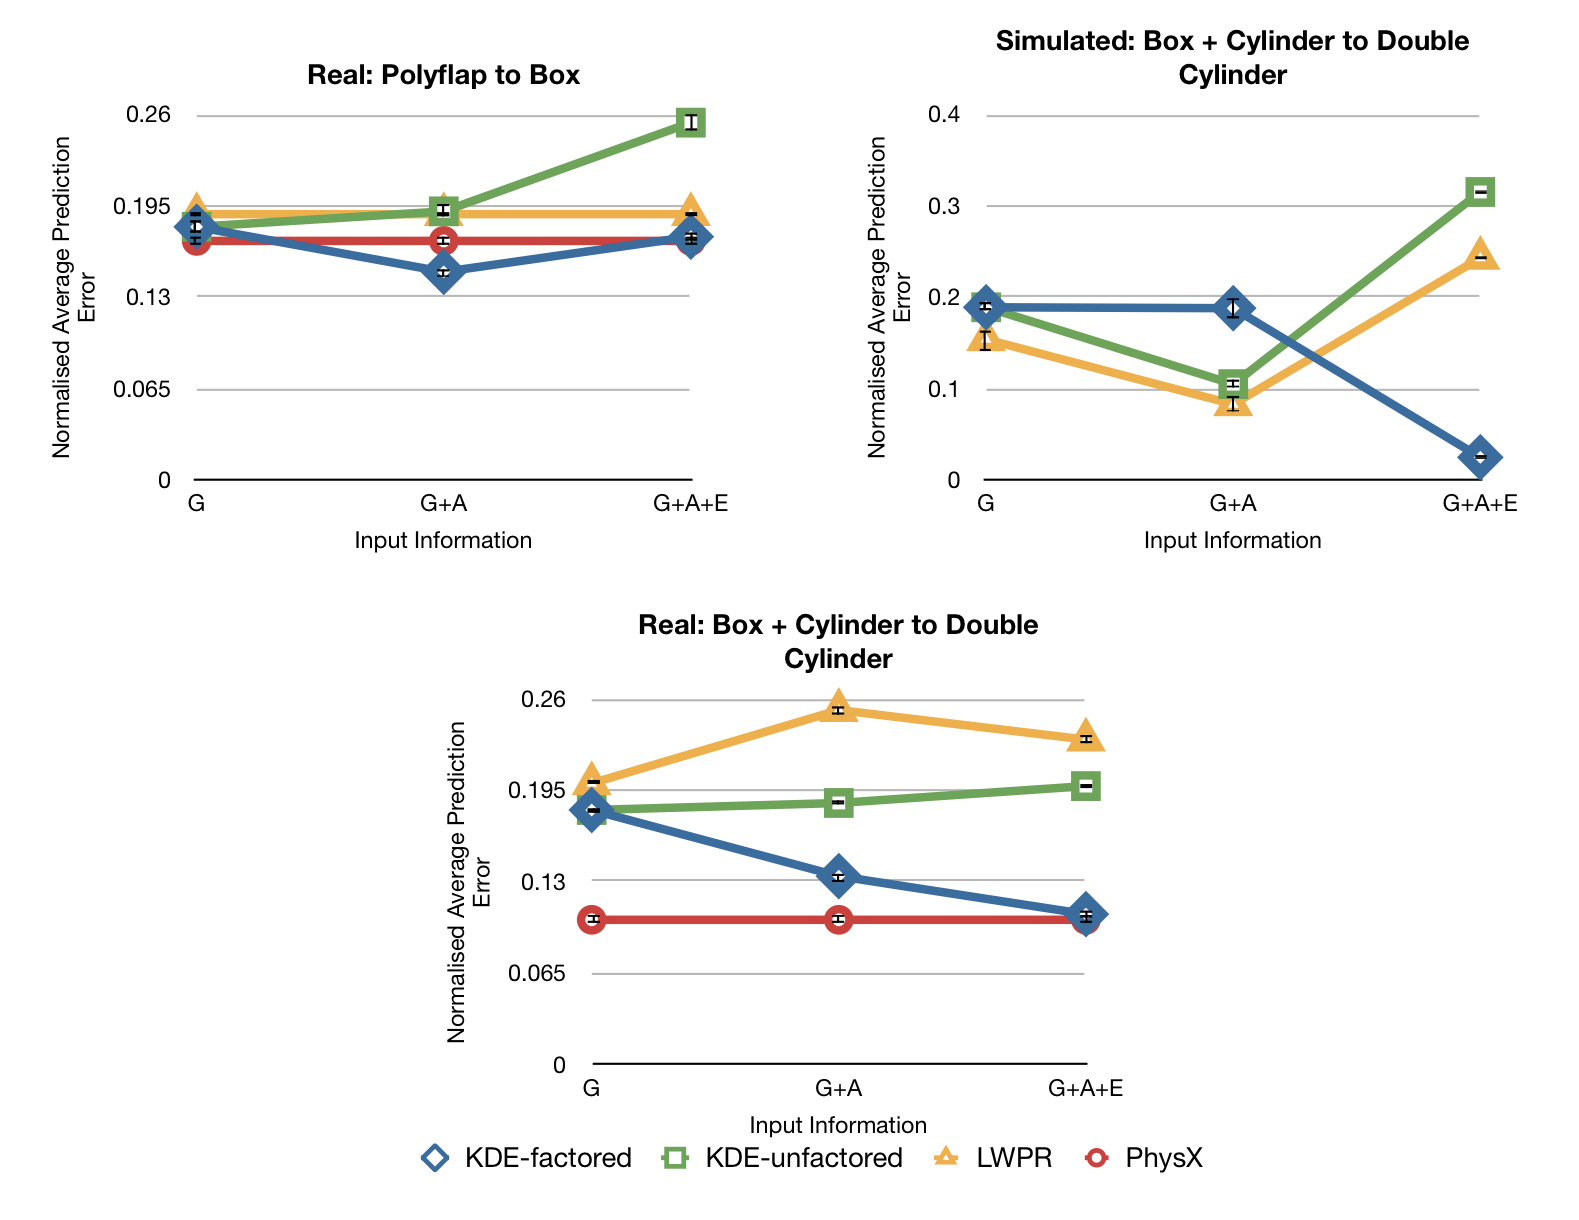
\includegraphics[width=\columnwidth]{graphs_jw/P3-graphs}}
\caption{Experiment P3: Comparative performance of predictors vs. information utilised, as measured by the normalised average error ${E_{av}^{norm}}$. 
}\label{fig:S_av_graphs}
\end{figure}

Related work is split into four broad areas: neuroscience, analytic approaches, qualitative physics and machine learning. Prediction of motor effects on the body has long been studied in neuroscience \cite{Miall1996,Flanagan2003}.  MOSAIC was an early computational model of prediction and control in the cerebellum using a modular scheme \cite{Haruno_MOSAIC_2008}, where predictions can be made by convex combinations of learned predictors. Other bio-inspired modular prediction schemes were independently derived by roboticists \cite{demiris2006hierarchical}. These models all differ from ours in that our work is the first attempt at modelling the motions of objects with kinematic constraints. There is also evidence that infants can learn object specific motions\cite{Bahrick1995}. It is also clear that while some object knowledge may be innate \cite{spelke1994early}, object specific predictions must learned, and are critical to our manipulation skills \cite{Flanagan2006}. So in general terms modular learning of predictions of object behaviour is cognitively plausible.

There is substantial work in robotics on classical analytic mechanics models of pushing \cite{mason_manipulator_1982,lynch_mechanics_1992,peshkin_motion_1988,cappelleri_designing_2006}, on both kinematic and dynamic models of manipulation effects \cite{mason_mechanics_2001}. Such analytic models are good predictors if their key parameters (e.g. friction) are precisely known. They can also inform push planning under pose uncertainty \cite{brost1985planning}. There is a separate body of work on qualitative models of action effects on objects, rooted in naive physics \cite{hayes1995second}, and qualitative physics \cite{kuipers1986qualitative}. In a similar spirit there is work on using physics engines to learn qualitative action effects \cite{Mugan-tamd-12}, and high level planning of manipulation \cite{stillman08ijrr,roy2004mental} using qualitative action models. Some early ideas on push planning have reappeared in recent robots that plan pushes to enable grasps in clutter \cite{Dogar_2010}.

At the other end of the spectrum machine learning can classify object behaviour by finding correlations between motions and global shape features \cite{fitzpatrick_learning_2003,ridge2010self}. The learning is similar in spirit, but produces classifiers, not predictors. Stoytchev \cite{Stoytchev_affordances_2008} is an example of convergence of the planning and learning themes, and closest in spirit overall to ours. A robot learns action effects of sticks and hook-like tools by pushing objects. This work is impressive, but simplifies the domain by using circular pucks as objects, and four planar motions as actions. Action outcomes were learned for various tools in a modular fashion, but without transfer learning.  

Our work sits at the intersection of some these approaches. We embrace machine learning and modularity to achieve scalability, but we also explicitly model each contact constraint. In this way we try to re-achieve in a machine learning framework what only the analytic approach has attempted to date: metric prediction of motion transferable to novel actions and objects. We avoid analytic modelling, to avoid the difficulties of parameter estimation. Thus we combine modelling of kinematic constraints with machine learning based approaches to provide a hybrid solution to prediction for manipulation.